
\medskip
Dans la figure ci-dessous, on a tracé $\mathcal{C}_f$ la courbe représentative d'une fonction $f$  définie et dérivable sur $\R$ ainsi que les tangentes à $\mathcal{C}_f$ aux points d'abscisses respectives $- 2$,\:$- 1$ et $0$.

\begin{center} 

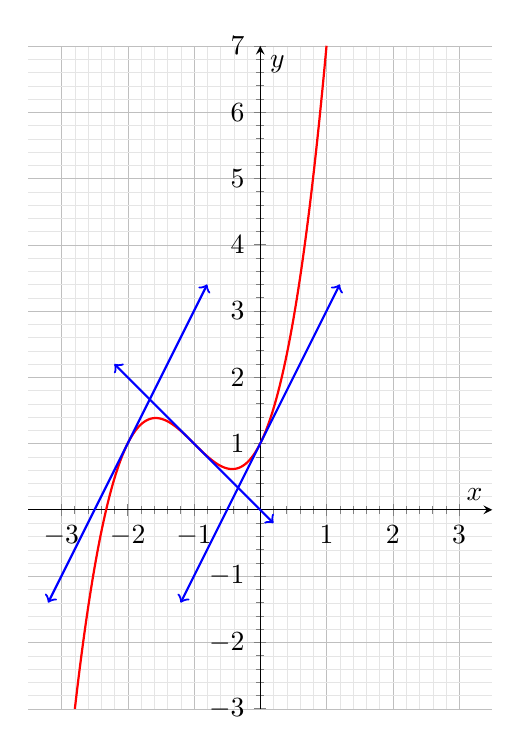
\begin{tikzpicture}
  \begin{axis}[
    width=15cm, % Largeur du graphique
    height=10cm, % Hauteur du graphique
    grid=both,
    grid style={line width=.1pt, draw=gray!50}, % Grille principale
    minor grid style={line width=.05pt, draw=gray!20}, % Sous-grille
    minor tick num=4, % Sous-grille tous les 0.2
    axis equal image, % Même échelle pour x et y
    axis lines=middle,
    xlabel={$x$}, ylabel={$y$},
    xmin=-3.5, xmax=3.5, % Limites sur l'axe des abscisses
    ymin=-3, ymax=7, % Limites sur l'axe des ordonnées
    xtick={-3,-2,...,3}, % Graduation des entiers sur l'axe x
    ytick={-3,-2,...,7}, % Graduation des entiers sur l'axe y
    enlargelimits=false,
    domain=-3:1,
    samples=200
  ]

    % Fonction principale
    \addplot[red, thick, no markers] {x^3 + 3*x^2 + 2*x + 1};

    % Tangente en x = -2
    \addplot[blue, thick, domain=-3.2:-0.8, <->] {
      (-2)^3 + 3*(-2)^2 + 2*(-2) + 1 + (3*(-2)^2 + 6*(-2) + 2)*(x - -2)
    };

    % Tangente en x = -1
    \addplot[blue, thick, domain=-2.2:0.2, <->] {
      (-1)^3 + 3*(-1)^2 + 2*(-1) + 1 + (3*(-1)^2 + 6*(-1) + 2)*(x - -1)
    };

    % Tangente en x = 0
    \addplot[ blue, thick, domain=-1.2:1.2, <->] {
      (0)^3 + 3*(0)^2 + 2*(0) + 1 + (3*(0)^2 + 6*(0) + 2)*(x - 0)
    };

  \end{axis}
\end{tikzpicture}

\end{center}


\begin{enumerate}
\item Recopier sur la copie en le complétant le tableau de valeurs ci-dessous. 

\begin{center}
\psset{unit=1cm,arrowsize=2pt 4}
\begin{tabularx}{0.5\linewidth}{|*{3}{>{\centering \arraybackslash}X|}}\hline
$x$		&$-1$	& $0$\\ \hline
$f(x)$	&		&\\ \hline
$f'(x)$	&		&\\ \hline
\end{tabularx}
\end{center}

On admet que la fonction $f$ est définie sur $\R$ par:

\[f(x) = x^3 +3x^2 +2x +1.\]

\item 
	\begin{enumerate}
		\item Calculer $f'(x)$, pour tout réel $x$.
		\item Résoudre dans $\R$ l'équation: $f'(x) = 0$.
	\end{enumerate}
\item Dresser le tableau de variations de la fonction $f$.

\item Le point S$(-4~;~-3)$ appartient-il à la tangente à la courbe représentative de $f$ au point d'abscisse $x = -2$ ?
\end{enumerate}

\bigskip

